\documentclass[TOTEM]{cern/cernphprep}

\usepackage{color}
\usepackage{enumitem}

%----------------------------------------------------------------------------

\def\d{{\rm d}}
\def\un#1{\,{\rm #1}}
\def\ung#1{\quad[{\rm #1}]}
\def\unt#1{[{\rm #1}]}
\def\e{{\rm e}}
\def\I{{\rm i}}
\def\T{{\rm T}}
\def\vec#1{\mathbf{#1}}
\def\mat#1{\mathsf{#1}}
\def\etal{et al.}
\def\todo#1{{\color{red}TODO: #1}}
\def\TODO#1{{\color{red}TODO: #1}}

\setbox123\hbox{$0$}
\setbox124\hbox{$.$}
\def\S{\hbox to\wd123{\hss}}
\def\.{\hbox to\wd124{\hss}}

\def\Name#1{#1, }
\def\Review#1#2#3#4{{\it #1} {\bf #2} (#3) #4}

\def\hang{\hangindent=\parindent}
\catcode`\>=11
\newskip\itskip \itskip2mm
\newskip\iitskip \iitskip0mm
\newdimen\itindent \itindent3mm
\newdimen\iitindent \iitindent5mm
\def\>{\par\vskip\itskip\parindent\itindent\indent\hang\llap{\hbox to3mm{$\bullet$\hss}}}
\def\>E{\par\vskip\itskip\parindent\itindent\indent\hang\llap{\hbox to3mm{\hss}}}
\def\>>{\par\vskip\iitskip\parindent\iitindent\indent\hang\llap{\hbox to\iitindent{\hss--\ }}}

%----------------------------------------------------------------------------------------------------

\begin{document}

\begin{titlepage}

\renewcommand{\EXPLOGO}{fig/logo_totem_black.pdf}

\PHnumber{TODO}
\PHdate{TODO}

\EXPnumber{TODO}
\EXPdate{TODO}

\title{Alignment of CT-PPS detectors in 2016, before TS2}

\ShortTitle{Alignment of CT-PPS detectors in 2016}

\author{Jan Ka\v spar}

\ShortAuthor{Jan Ka\v spar}

\begin{abstract}
TODO: abstract
\end{abstract}

%\centerline{version 0}	% sent on 19 Dec 2016
\centerline{version 2-pre}

\end{titlepage}

%----------------------------------------------------------------------------------------------------

\section{Introduction}
\label{s:intro}

\> why is the alignment important
\>> what is the desired precision, put in context with detector resolution and impact on xi uncertainty -- compared to other uncertainties.

Figure~\ref{fig:rp_layout} shows the layout of the RPs around IP5. The RPs marked in red are used by CT-PPS and will be of primary interest of this note. The vertical RPs in both $210\un{m}$ stations are also used for alignment purposes.

\begin{figure}[h!]
\begin{center}
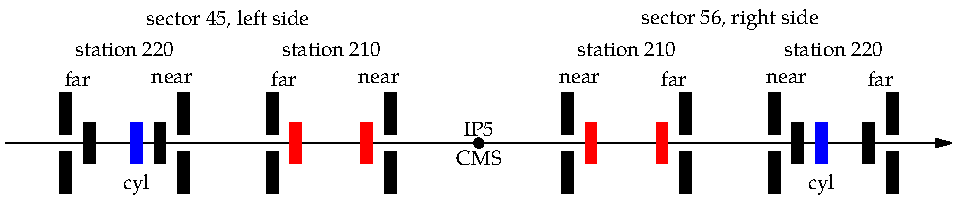
\includegraphics{fig/rp_layout.pdf}
\caption{%
Layout of RPs aroud IP5. The red RPs contain the tracking Si strips sensors used for CT-PPS. The blue RPs host the timing diamond sensors. The other RPs are used only by the TOTEM experiment.
}
\label{fig:rp_layout}
\end{center}
\end{figure}

This note describes the first alignment of CT-PPS data taken in 2016, before TS2 -- in the LHC fills 4947 through 5288. 

The alignment proceeds in the two following stages.
\begin{enumerate}[noitemsep]
\item Alignment is performed with data from a special low-luminosity calibration fill (4828), where both horizontal and vertical RPs are inserted very close to the beam (about $5\un{\sigma}$). The standard TOTEM procecure \cite{totem-ijmp} is used, details will be give in Section~\ref{s:calib}.
\item The alignment information is transferred from the calibration fill to the standard physics fills with high luminosity and only horizontal RPs inserted. This new procedure is described in Section~\ref{s:phys}.
\end{enumerate}

The alignment and optics calibration \cite{optics_calibration} is eventually followed by a reconstruction validation, see Section~\ref{s:val}.

\> \TODO{consistent use of ``fill'' and ``run''}

%----------------------------------------------------------------------------------------------------

\section{Alignment in calibration runs}
\label{s:calib}

\> calibration run: low intensity, both horizontal and vertical RPs inserted, all RPs close to the beam (\TODO{number of sigmas})

\> the standard ``TOTEM'' procedure -- Section 3.4 in \cite{totem-ijmp}

\> three steps
\>> beam-based alignment: prior to data-taking, RPs are moved to the same $n_\sigma$ distance as collimators, when RPs touch the sharp beam edge created by collimators, strong BLM signal is observed; see Figure 7 in \cite{totem-ijmp}
\>> track-based alignment: relative alignment among all silicon sensors, analysis of track-hit residuals; Section~\ref{s:calib-track}
\>> elastic-based alignment: absolute alignment wrt.~beam, using symmetries of elastic scattering; Section~\ref{s:calib-elastic}

%--------------------------------------------------
\subsection{Relative alignment among RP sensors}
\label{s:calib-track}

\> can use any track passing through the RP station

\> key point: overlap between horizontal and vertical RPs $\rightarrow$ relative alignment among all RPs

\begin{figure}[h!]
\begin{center}
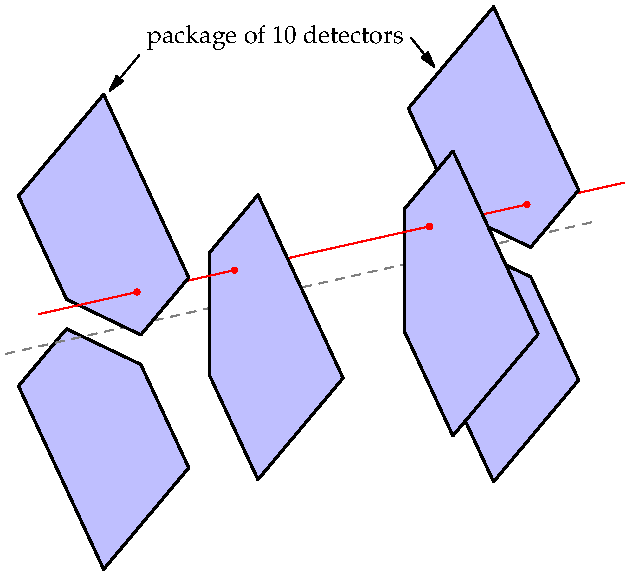
\includegraphics[width=5cm]{fig/rp_overlap.pdf}
\caption{%
A track (red line) passing through an overlap between vertical and horizontal RPs. The blue areas represent stacks of 10 Si strip sensors. The dashed black line indicates the beam.
}
\label{fig:rp_overlap}
\end{center}
\end{figure}

\> general method: analysis of track-hit residuals, see details in Section 4.2 in \cite{jan_thesis}
\>> optimisation of shift (in read-out direction) and rotation (about beam axis) of each Si sensor
\>> performed in several iterations (about 5), gradually imposing more strict track selection cuts as alignment precision improves
\>> not sensitive to certain (global) alignment modes (addressed in Section \ref{s:calib-elastic}): x and y shift and rotation of each unit (near or far) $\rightarrow$ optimising under constraint of zero mean global alignments
\>> applied to several sub-samples (TOTEM runs) for stability and systematics control

\> specific features
\>> 1 or 2 RPs missing in the right arm $\rightarrow$ complications, worse precision, even when using uMuMvRot=true

\> results can be decomposed into
\>> ``RP alignments'': alignments shared by all sensors in a RP
\>> ``internal alignments'': sensors alignments wrt.~the ``RP alignments''

\> examples
\>> Figure \ref{fig:tb_residuals}: residuals become centred about 0 during the procedure
\>> Figure \ref{fig:tb_example_internal}: example of ``internal alignments'', very good stability
\>> Figure \ref{fig:tb_example_rp}: example of ``RP alignments'', very good stability

\begin{figure}[h!]
\begin{center}
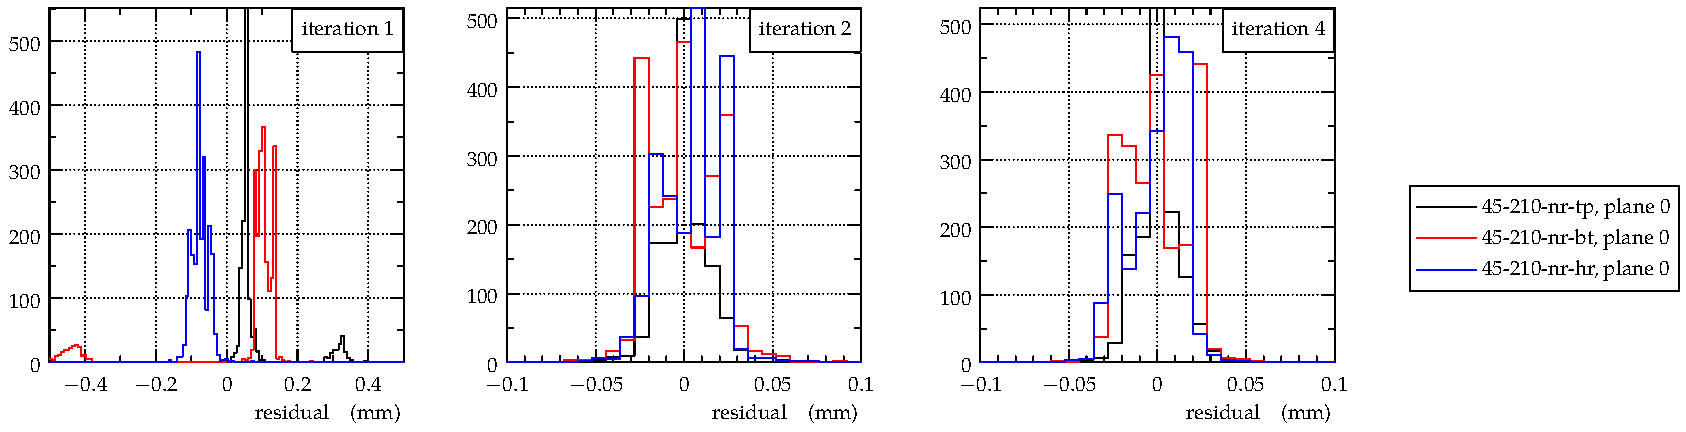
\includegraphics[width=\hsize]{fig/calibration_fill/residuals.pdf}
\caption{%
Distributions of track-hit residuals (TOTEM run 10332, after TS2). Each colour corresponds to a different sensor (first planes in the RPs of the 45-210-nr unit). The blue histogram has been downscaled by factor 100. {\it Left}: before any optimisation. The disconnected histogram portions originate from different RP configurations contributing to the track fit. {\it Middle}: after shift optimisation. {\it Right}: after shift and rotation optimisation.
}
\label{fig:tb_residuals}
\end{center}
\end{figure}

\begin{figure}[h!]
\begin{center}
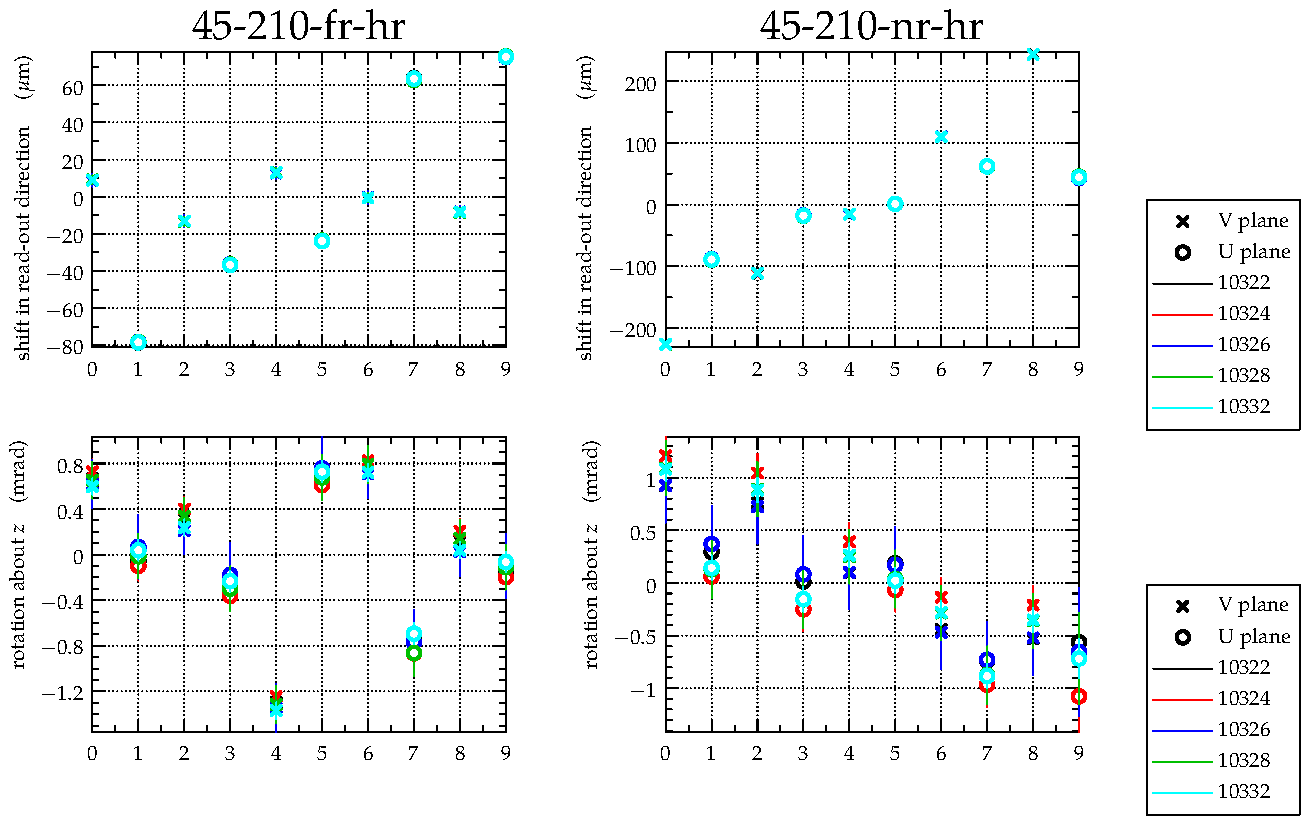
\includegraphics[width=0.8\hsize]{fig/calibration_fill/plots_per_plane_left.pdf}
\caption{%
Comparison of internal alignments obtained from different TOTEM runs (different colours), for the period after TS2. The two columns correspond to the two horizontal RPs in the sector 45. The horizontal scale gives the plane index within the detector package: 0 is the closest to the IP, 9 the farthest. The results for ``V'' (``U'') planes are marked with crosses (circles). The linear patterns in the determined shifts (separately in ``U'' and ``V'' projections) can be understood by tilts of the entire detector package which shift the sensor centre's proportionally to its position within the package, for more details see Section 4.2.8 in \cite{jan_thesis}. The error bars indicate statistical uncertainties only.
}
\label{fig:tb_example_internal}
\end{center}
\end{figure}

\begin{figure}[h!]
\begin{center}
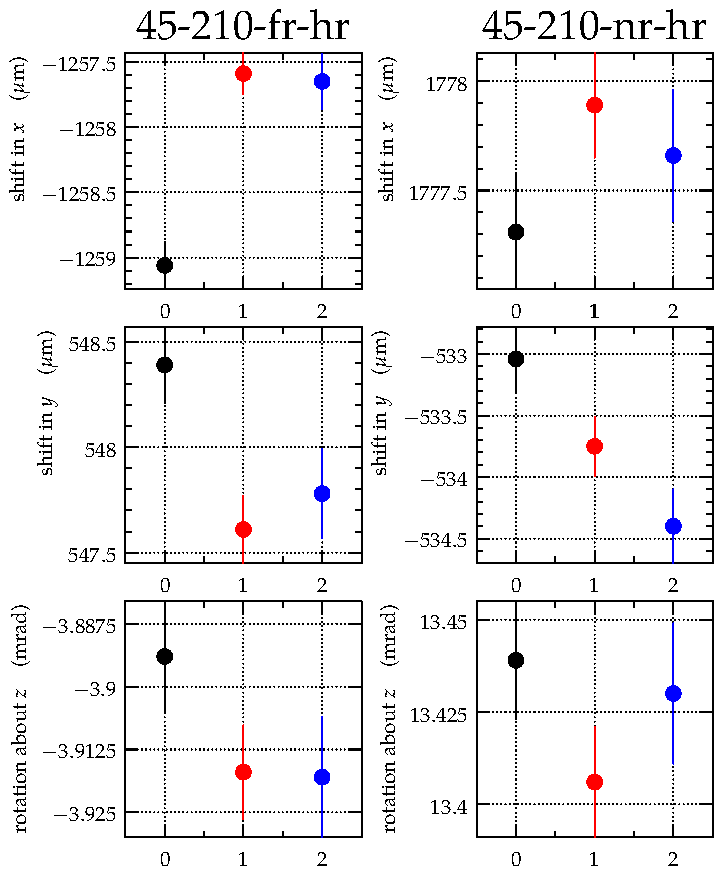
\includegraphics[width=0.8\hsize]{fig/calibration_fill/plots_per_rp_left.pdf}
\caption{%
Comparison of ``RP'' alignments obtained from different TOTEM runs (different colours), for the period after TS2. The two columns correspond to the two horizontal RPs in the sector 45. The error bars indicate statistical uncertainties only.
}
\label{fig:tb_example_rp}
\end{center}
\end{figure}


\> uncertainties
\>> statistical uncertainties estimated by the algorithm
\>> systematic uncertainties inferred from the difference between sub-samples, see Figures \ref{fig:tb_example_internal} and \ref{fig:tb_example_rp}.
\>> combined uncertainties:
\>> before TS2 -- \TODO{values}
\>> after TS2 -- left arm: $5\un{\mu m}$ for shifts, $0.3\un{mrad}$ for rotations, right arm: $25\un{\mu m}$ for shifts, $1\un{mrad}$ for rotations 


%--------------------------------------------------
\subsection{Absolute alignment with respect to the beam}
\label{s:calib-elastic}

\> missing RPs in the right arm
\>> non-optimal $\theta_x^*$ reconstruction
\>> reduced number of elastic selection cuts

\> elastic selection cuts
\>> $\theta_x^*$ left-right collinearity, see Figure \ref{fig:el_cuts}, top left.
\>> $\theta_y^*$ left-right collinearity, see Figure \ref{fig:el_cuts}, top right.
\>> $x^*$ in the left compatible with vertex distribution, see Figure \ref{fig:el_cuts}, bottom left.
\>> position-angle correlation in $y$ plane in the left arm, see Figure \ref{fig:el_cuts}, bottom right.

\begin{figure}[h!]
\begin{center}
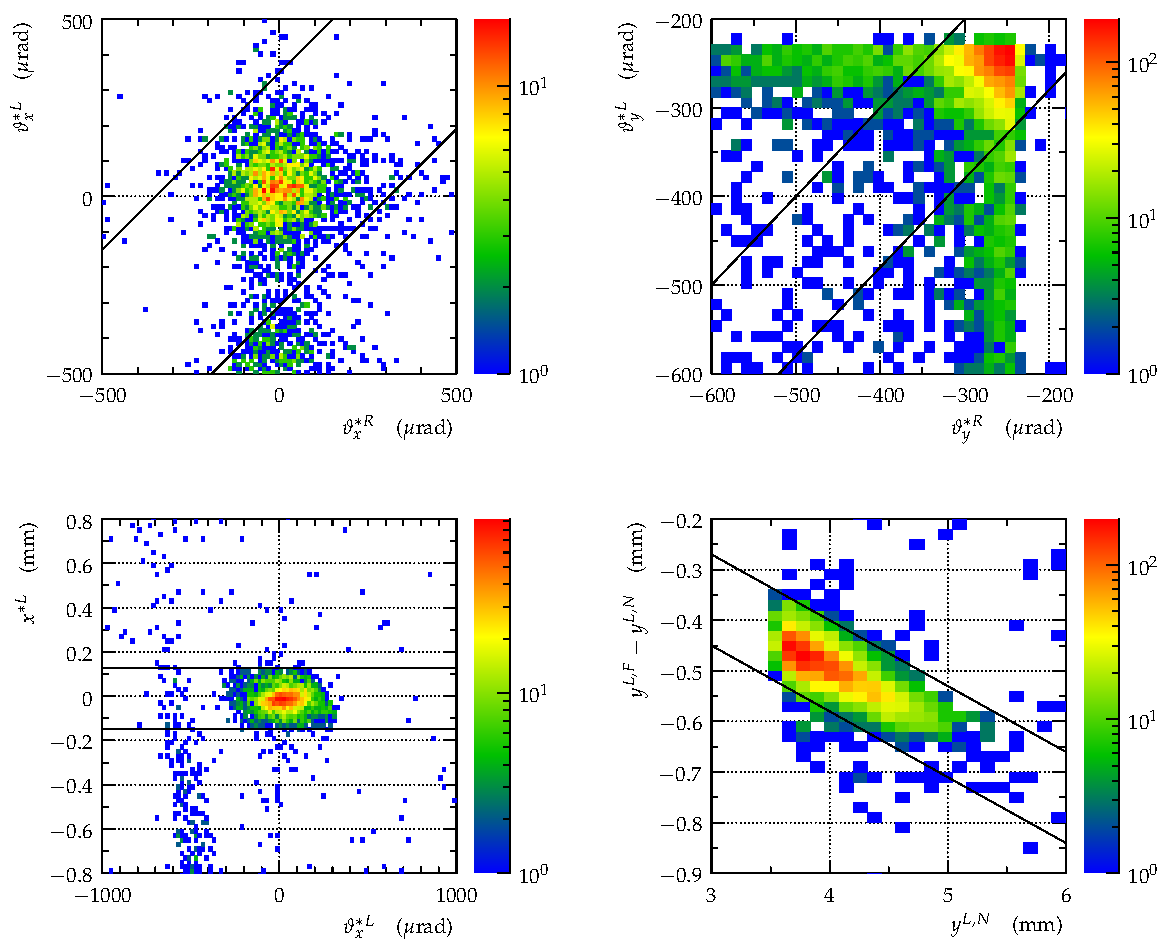
\includegraphics[width=0.8\hsize]{fig/calibration_fill/el_cut_example.pdf}
\caption{%
Example of elastic selection cuts, for period before TS2. The black lines delimit the selection region.
}
\label{fig:el_cuts}
\end{center}
\end{figure}

\> method: describe Figure \ref{fig:el_alignment_method}
\>> applied to 1h time slices -- examine time variation, systematics

\begin{figure}[h!]
\begin{center}
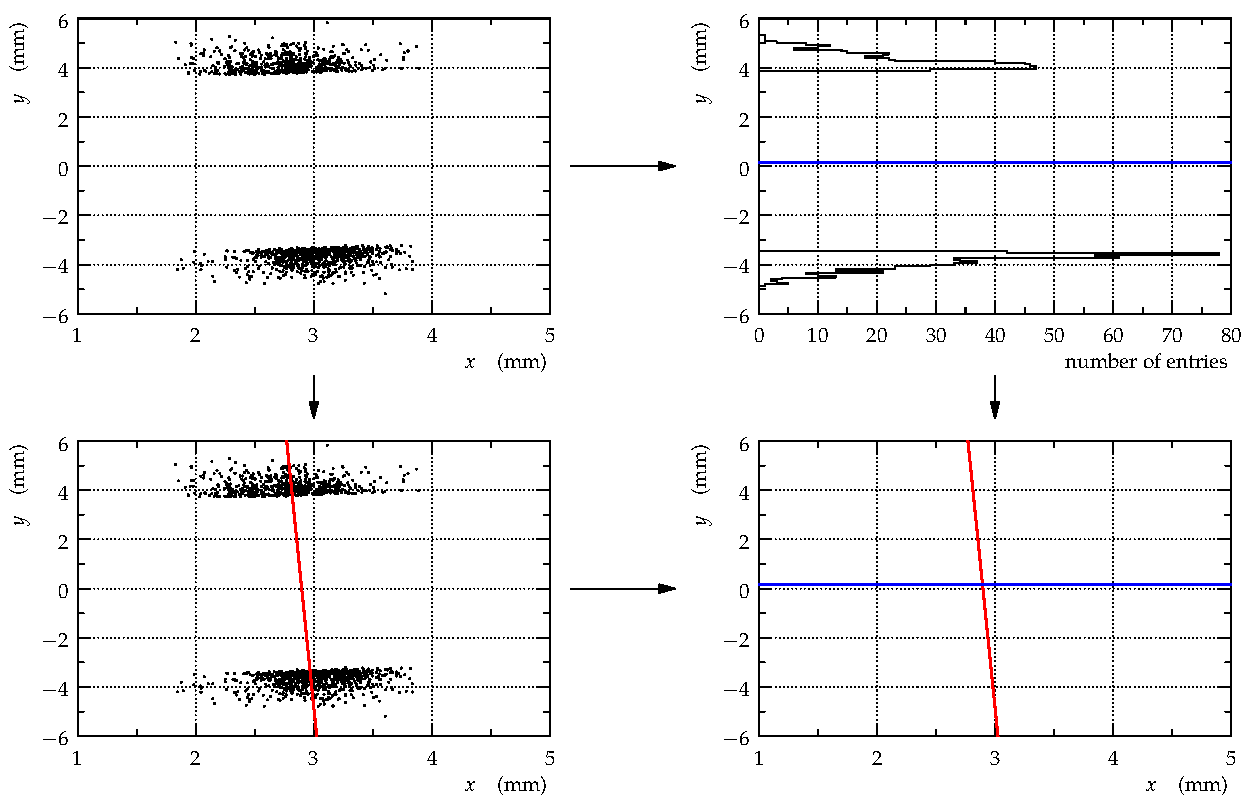
\includegraphics[width=0.7\hsize]{fig/calibration_fill/el_alignment_method.pdf}
\caption{%
Illustration of alignment with elastic scattering. Data from a 1h-slice of pre-TS2 data.
}
\label{fig:el_alignment_method}
\end{center}
\end{figure}

\> describe the several metrics for each alignment variable

\> exception: RP 56-210-nr-tp not available
\>> had to fix the tilt: to similar value as in the far top RP
\>> no vertical alignment for this RP -- \TODO{try by equalising theta y from different RPs}

\> Figure \ref{fig:el_alignment_results}: summary of results

\begin{figure}[h!]
\begin{center}
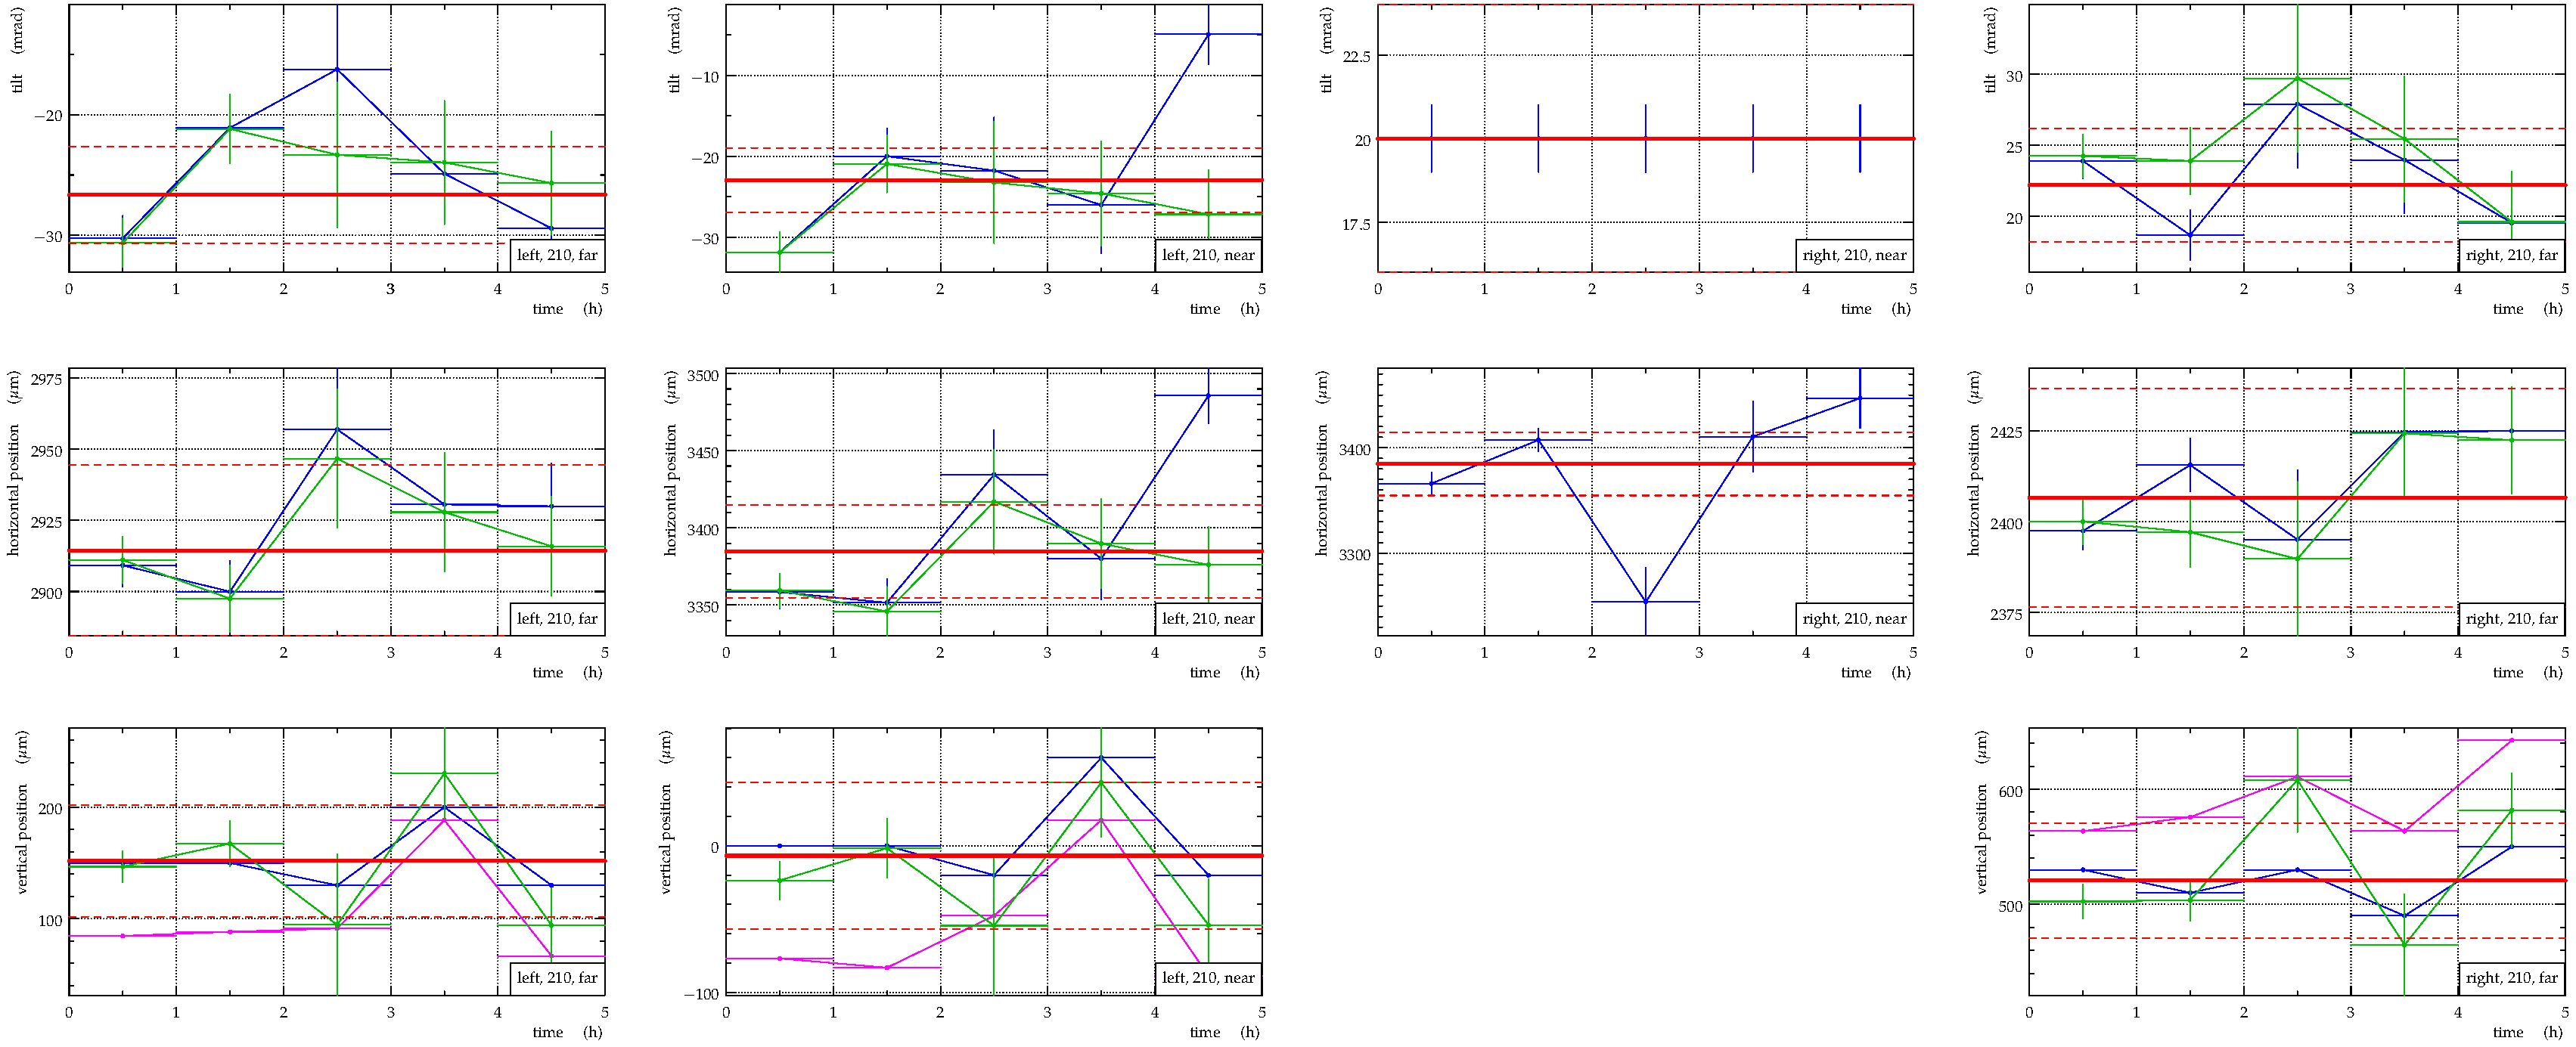
\includegraphics[width=\hsize]{fig/calibration_fill/el_alignment.pdf}
\caption{%
Summary of the elastic-alignment results in the period before TS2. Each column corresponds to one RP unit. The rows (top to bottom) show: tilt (about the beam axis), horizontal beam position and vertical beam position. \TODO{Keep just one line/metric per quantity}? The red solid (dashed) lines denote the final extracted values \TODO{how?} (their uncertainties)
}
\label{fig:el_alignment_results}
\end{center}
\end{figure}

%----------------------------------------------------------------------------------------------------

\section{Alignment in physics runs}
\label{s:phys}

\> basic idea: the physics is the same for all runs

\> if optics, ... not changed, then also physics hit distributions equal for all runs

\> alignment method: match/align physics hit distributions from physics runs to the calibration run

\> event selection
\>> CMS trigger: $\sim$ zero bias for RPs
\>> physics protons (coming from IP): strong correlation $x^{\rm F}$ vs.~$x^{\rm N}$, see Figure \ref{fig:hor_cuts}.

\begin{figure}[h!]
\begin{center}
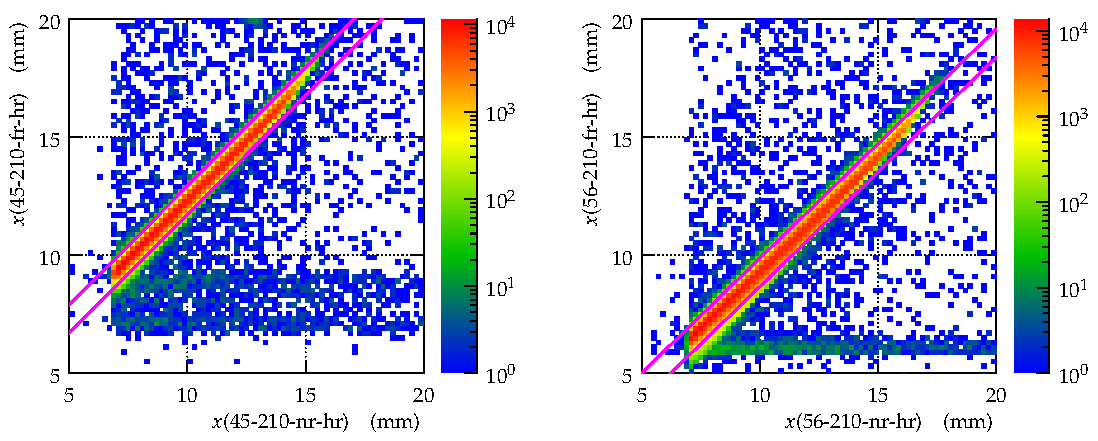
\includegraphics[width=0.7\hsize]{fig/physics_fills/hor_cuts.pdf}
\caption{%
Example of cleaning cuts, employing the correlation between the horizontal track positions in the near and far RP of each station. Data from a sub-sample of the pre-TS2 period.
}
\label{fig:hor_cuts}
\end{center}
\end{figure}

\> the effect of the cleaning cuts: Figure \ref{fig:hor_cuts_effect}

\begin{figure}[h!]
\begin{center}
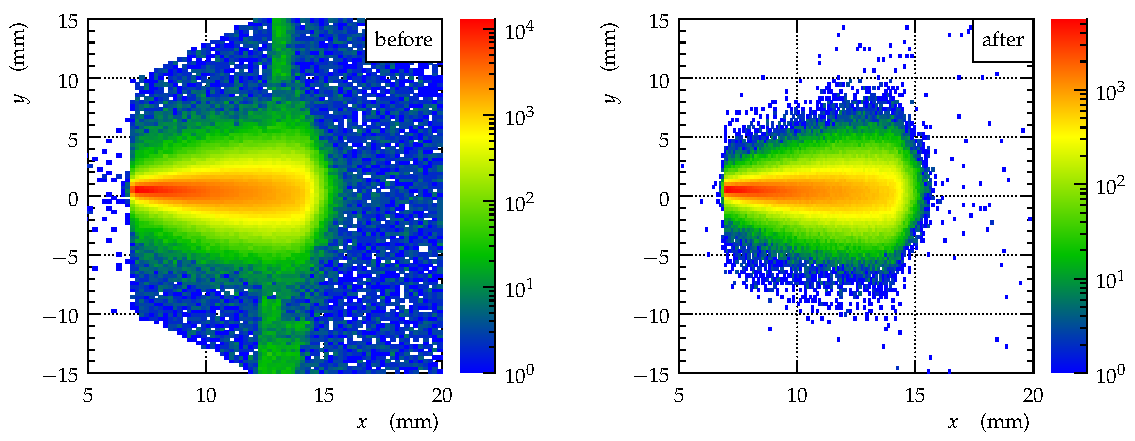
\includegraphics[width=0.7\hsize]{fig/physics_fills/hor_cuts_effect_cmp.pdf}
\caption{%
Illustration of the effect of the cleaning cuts presented Figure~\ref{fig:hor_cuts}. {\it Left}: hit distribution in \TODO{which RP} before applying the cuts, {\it right}: the same distribution after the cuts. Data from a sub-sample of the pre-TS2 period.
}
\label{fig:hor_cuts_effect}
\end{center}
\end{figure}

%--------------------------------------------------
\subsection{Conditions}

\> RP insertions
Figure~\ref{fig:cond_rp}

\begin{figure}[h!]
\begin{center}
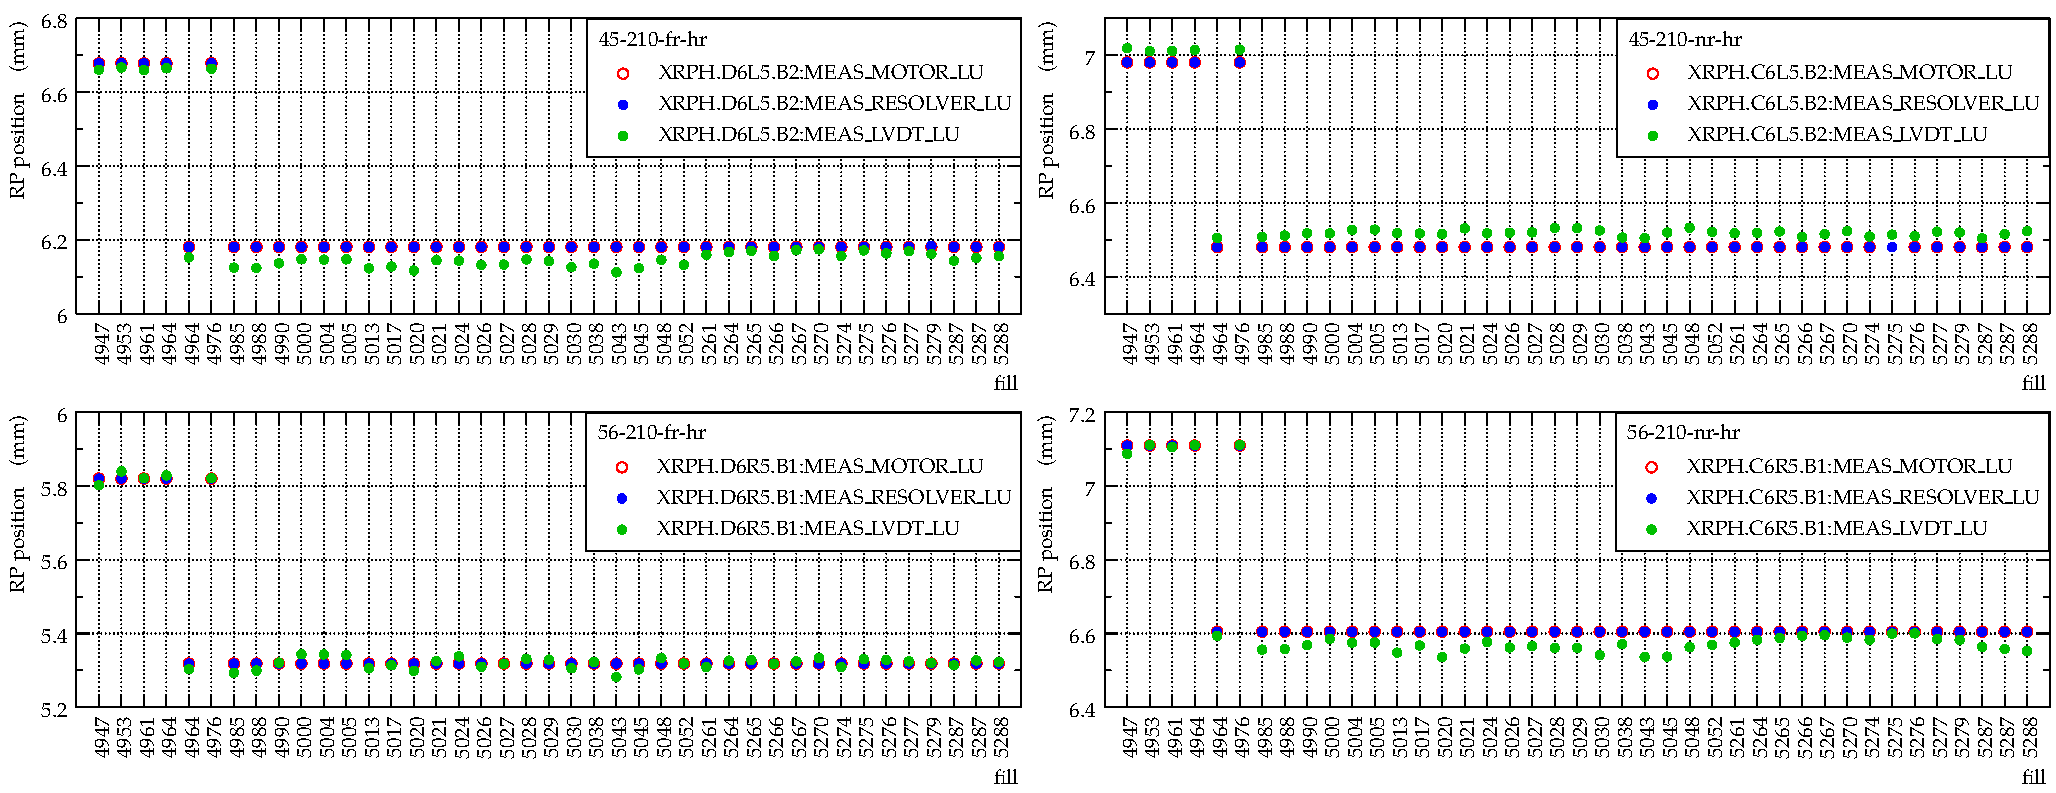
\includegraphics[width=1\hsize]{fig/conditions/rp_positions_rps.pdf}
\caption{%
RP positions as reported by the 3 position gauges (LVDT, MOTOR and RESOLVER) per LHC fill (horizontal axes). The two entries for fill 4964 correspond to the insertions with and without safety margin. The two entries for fill 5287 correspond to the two insertions within the same fill.
}
\label{fig:cond_rp}
\end{center}
\end{figure}


\> BPM measurements of the orbit
Figure~\ref{fig:cond_bpm}

\begin{figure}[h!]
\begin{center}
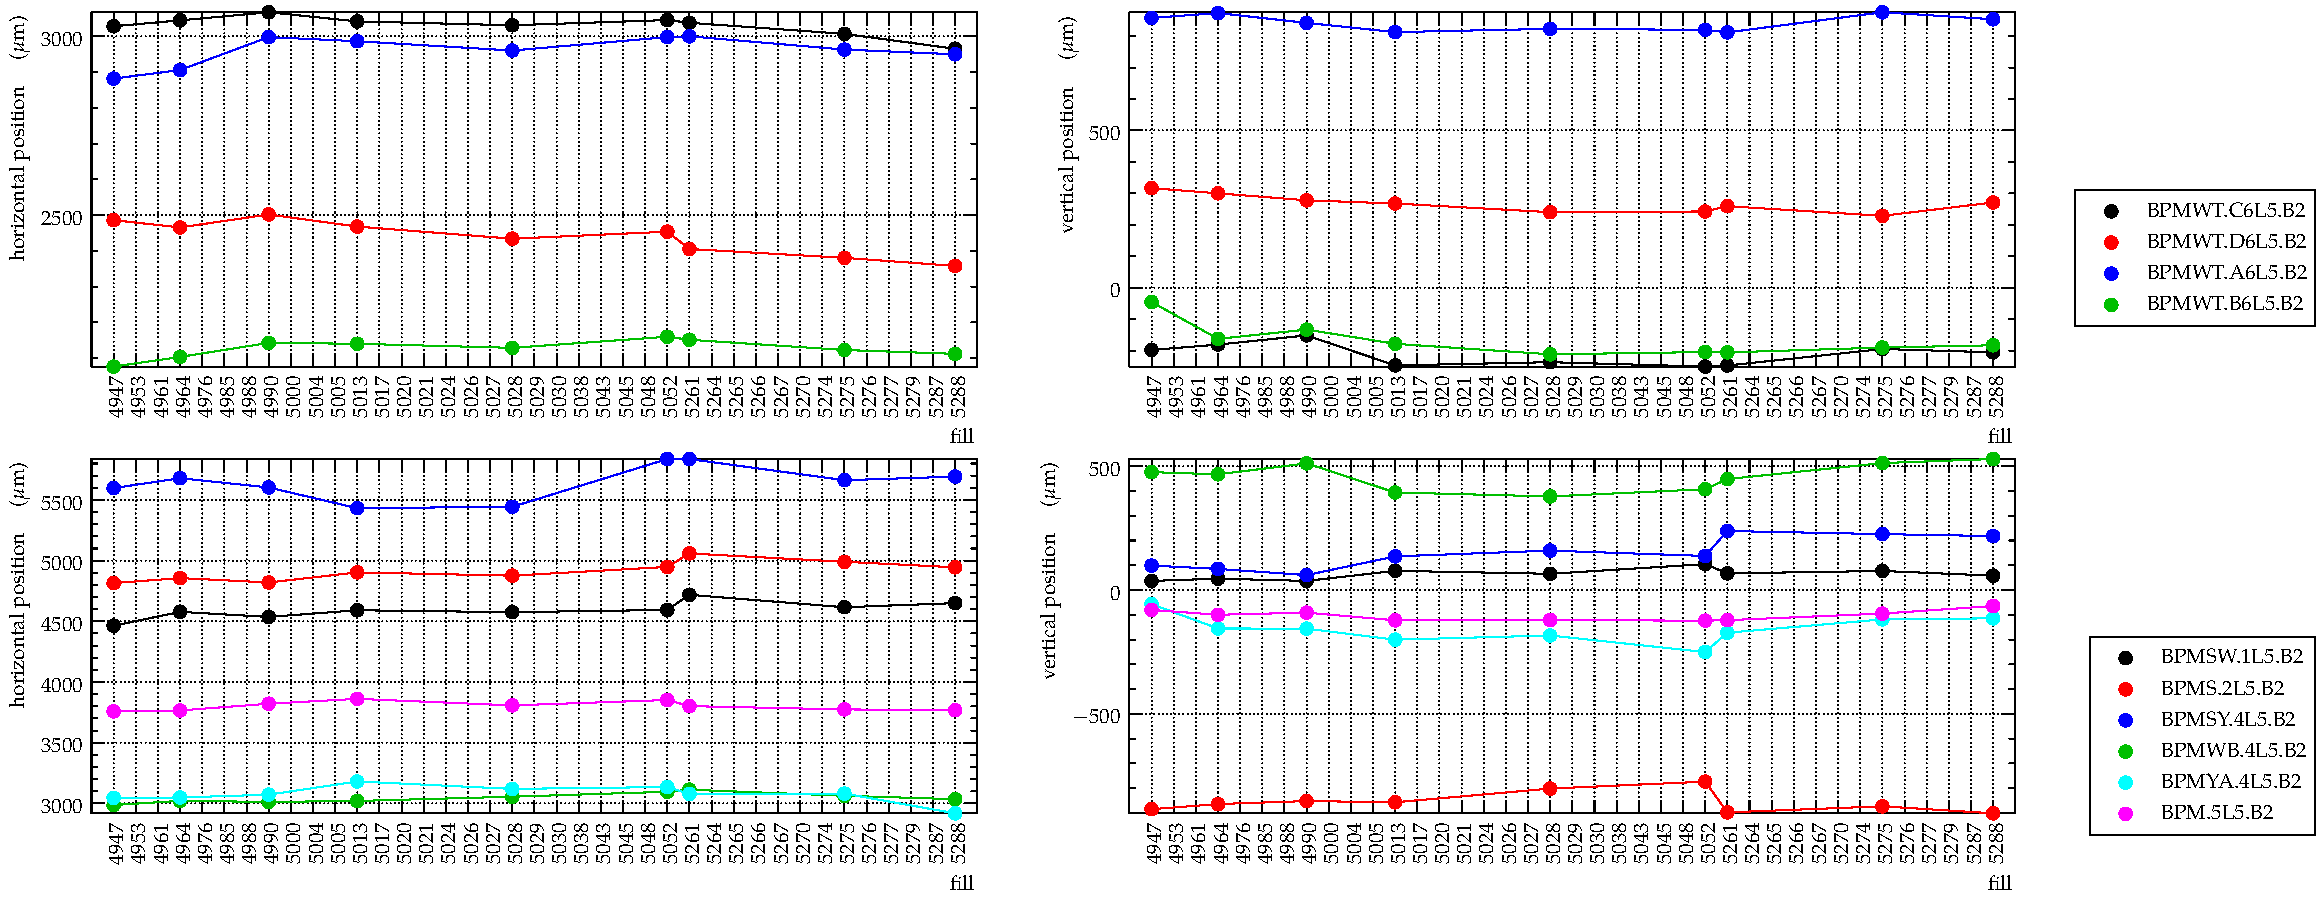
\includegraphics[width=1\hsize]{fig/conditions/bpm_comparison.pdf}
\caption{%
Readings of BPMs close to the RP stations in a selection of LHC fills of interest. The monitors C6, D6, A6 and B6 correspond to RP units 210-nr, 210-fr, 220-nr and 220-fr, respectively.
}
\label{fig:cond_bpm}
\end{center}
\end{figure}


\> collimator positions
Figure~\ref{fig:cond_collimators}

\begin{figure}[h!]
\begin{center}
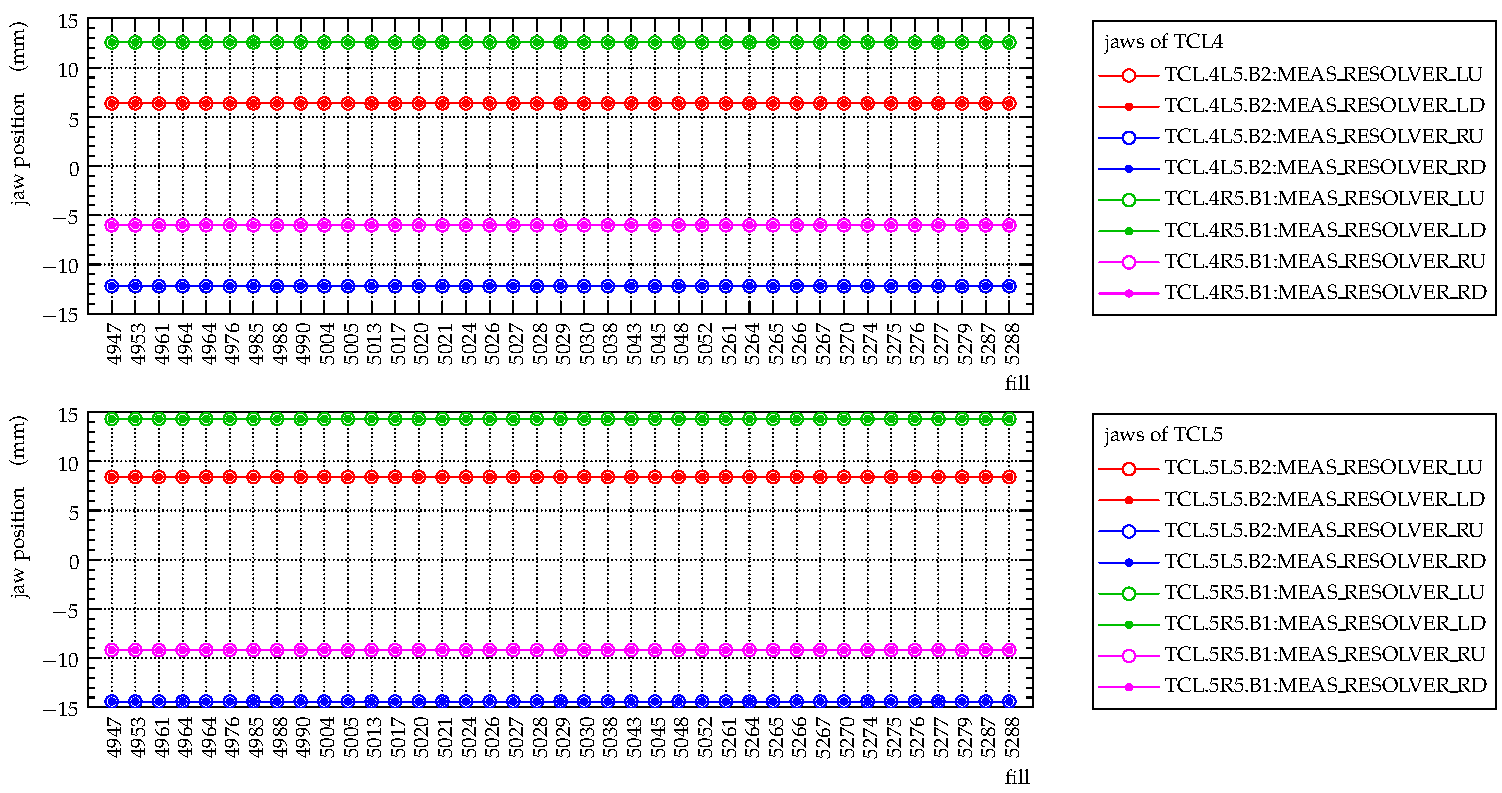
\includegraphics[width=1\hsize]{fig/conditions/collimator_positions_resolver.pdf}
\caption{%
Positions of the relevant collimator jaws as a function of LHC fill. The left/right entry for fill 4964 corresponds to the insertion with/without the safety margin. The variable names (see legend) containing B1 (B2) correspond to collimators in beam 1 (beam 2). The last two characters of the variable name indicate the jaw: L stands for left, R for right, U for upstream and D for downstream.
}
\label{fig:cond_collimators}
\end{center}
\end{figure}


%--------------------------------------------------
\subsection{Horizontal alignment}

\> describe the to matching metrics
\>> describe the pros and cons of each
\>> Figure \ref{fig:hor_match_method}

\begin{figure}[h!]
\begin{center}
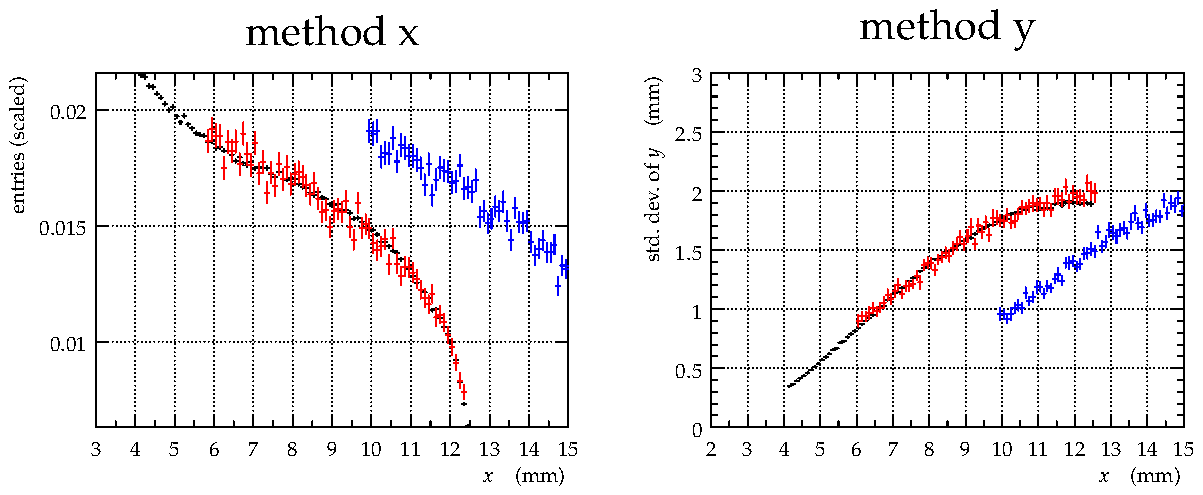
\includegraphics[width=0.7\hsize]{fig/physics_fills/match_method_example.pdf}
\caption{%
Illustration of the match metrics used for horizontal alignment, for a sub-sample from the pre-TS2 period. Black histogram: reference from the calibration fill. Blue (red) histogram: distribution from a physics fill before (after) matching.
}
\label{fig:hor_match_method}
\end{center}
\end{figure}

\> results: summarised in Figure \ref{fig:hor_match_results}
\>> \TODO{describe, comment}
\>> \TODO{add also method y results?} 

\begin{figure}[h!]
\begin{center}
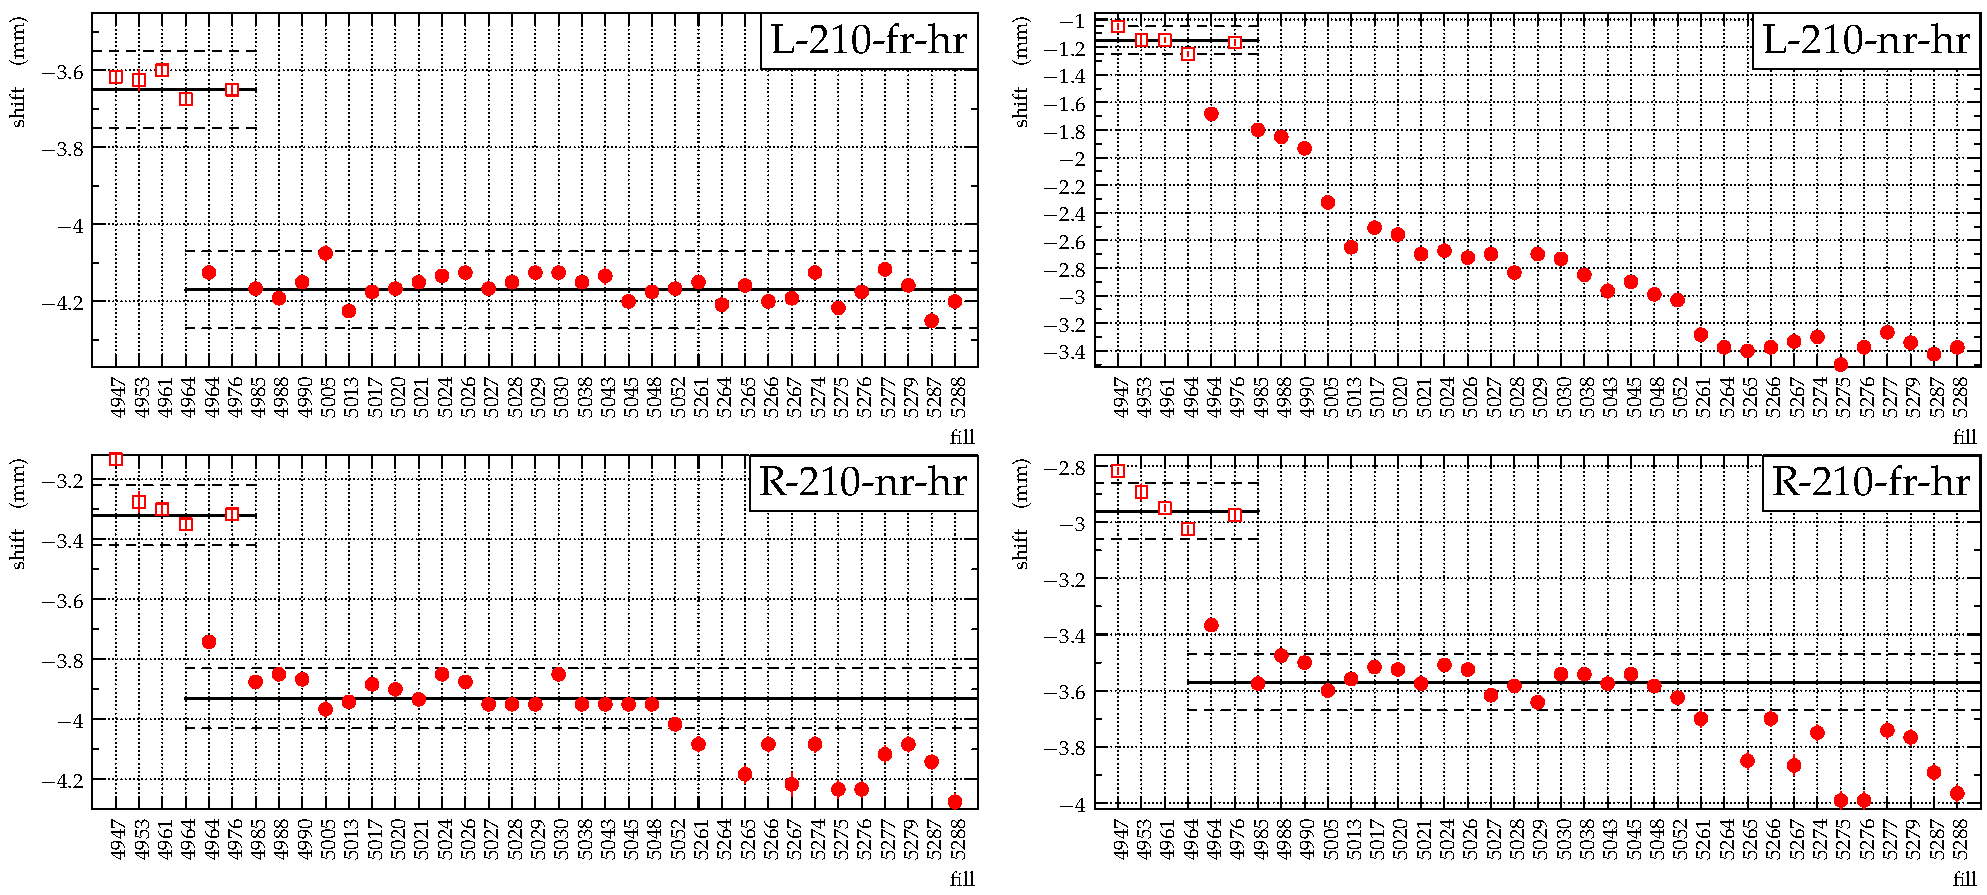
\includegraphics[width=\hsize]{fig/physics_fills/match_result_cmp_mean.pdf}
\caption{%
Summary of the horizontal-shift results. The horizontal axis indicates the fill number, the vertical scale gives the correction by how much the hit distribution should be moved.
}
\label{fig:hor_match_results}
\end{center}
\end{figure}

\> \TODO{comment on 45-210-nr-hr ...}


%--------------------------------------------------
\subsection{Vertical alignment}

\> yet to be done...

\> we may not need it for this note: it is not essential for $\xi$ reconstruction

%----------------------------------------------------------------------------------------------------

\section{Alignment and optics validation}
\label{s:val}

\> basic idea: the physics is RP-independent, each RP should see (up to acceptance, resolution, etc.) the same physics

\> in addition: can compare $\xi$'s within each arm on event-to-event basis

\> \TODO{which alignment results used}

\> $\xi$ is reconstructed pot-by-pot using $x$ to $\xi$ curves from the optics-calibration study \cite{optics_calibration}

\> \TODO{specify whether cleaning cuts are used}

\> \TODO{add $\xi$ correlation plot: near vs.~far RP}

\> Figure \ref{fig:xi_cmp_run}: fill-to-fill stability
\>> \TODO{describe}

\begin{figure}[h!]
\begin{center}
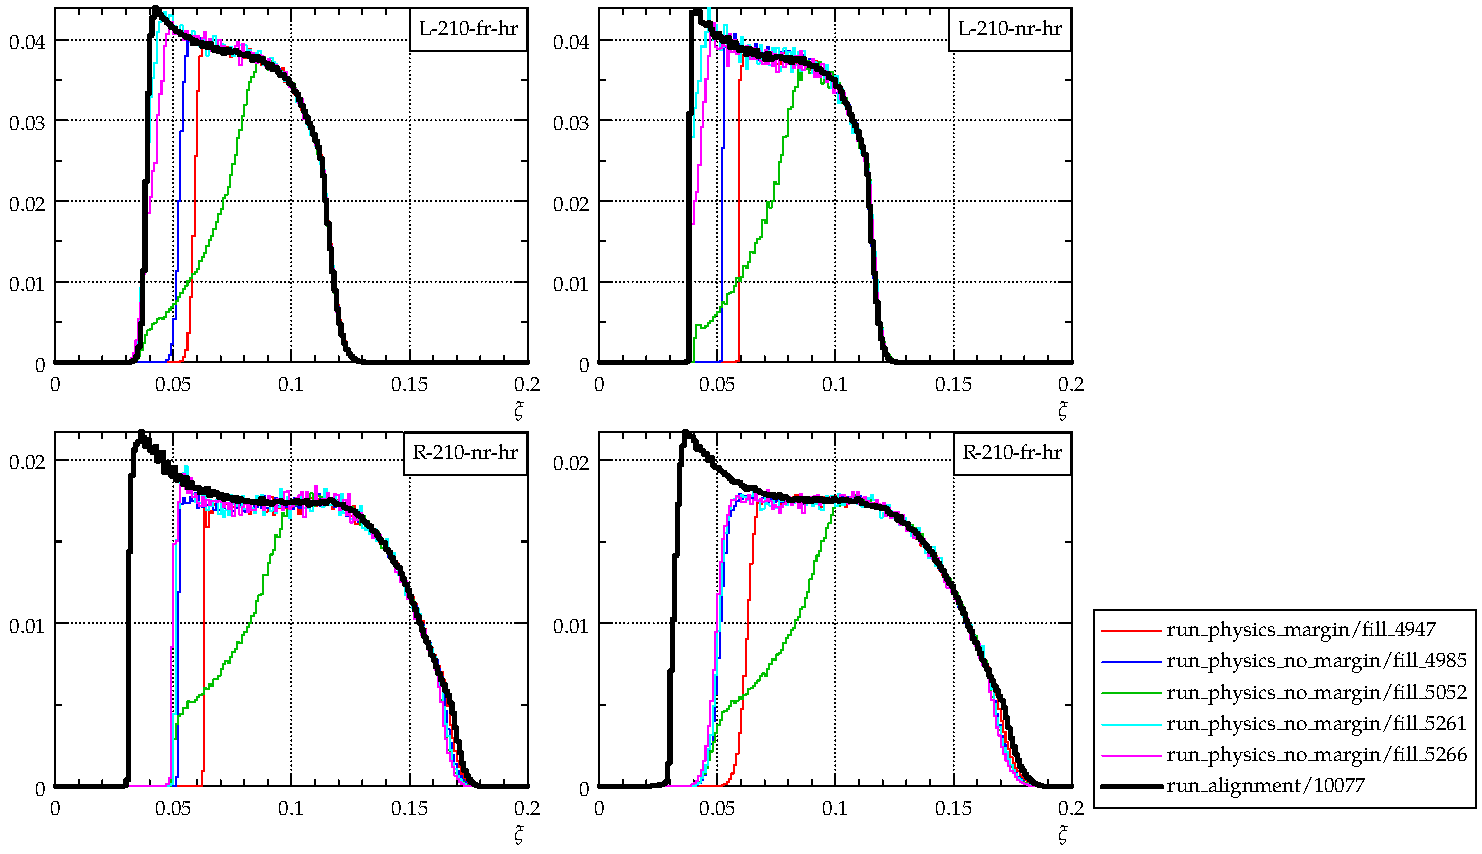
\includegraphics[width=0.7\hsize]{fig/validation/xi_cmp_run.pdf}
\caption{%
Fill-to-fill comparison of $\xi$ distributions extracted from single RPs. \TODO{describe the effects of radiation damage}
}
\label{fig:xi_cmp_run}
\end{center}
\end{figure}


\> Figure \ref{fig:xi_cmp_rp}: comparison of $\xi$ distributions from different RPs
\>> \TODO{comment}

\begin{figure}[h!]
\begin{center}
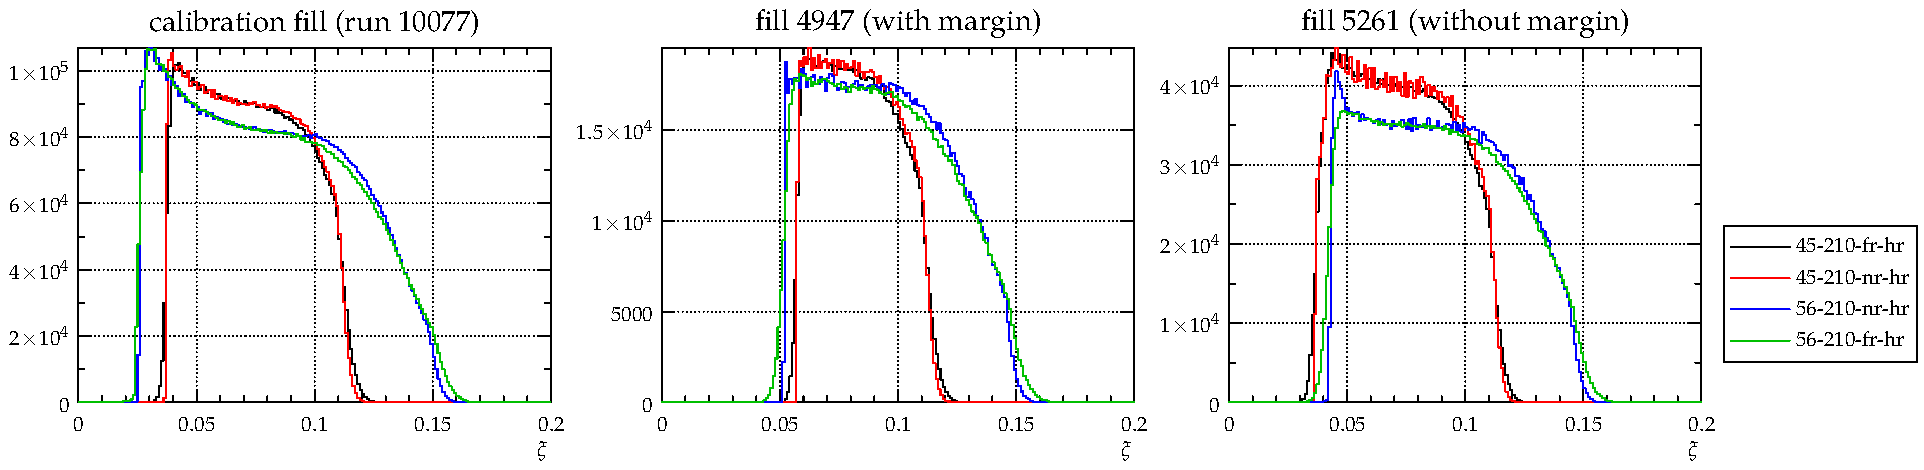
\includegraphics[width=0.7\hsize]{fig/validation/xi_cmp_rp.pdf}
\caption{%
Comparison of $\xi$ distributions from different RPs.
}
\label{fig:xi_cmp_rp}
\end{center}
\end{figure}



%----------------------------------------------------------------------------------------------------

\section{Summary}
\label{s:sum}

\> \TODO{TODO}

%----------------------------------------------------------------------------------------------------

\begin{thebibliography}{99}

\bibitem{totem-jinst}
	\Name{G.~Anelli \etal{}~(TOTEM Collaboration)}
	\Review{JINST}{3}{2008}{S08007}.
    %The TOTEM Experiment at the CERN Large Hadron Collider, JINST 3 S08007, 2008

\bibitem{totem-ijmp}
	\Name{G.~Antchev \etal{}~(TOTEM Collaboration)}
	\Review{Int.~J.~Mod.~Phys.~A}{28}{2013}{1330046}.

\bibitem{jan_thesis}
	\Name{J.~Ka\v spar}
	PhD Thesis, CERN-THESIS-2011-214,
	\url{http://cdsweb.cern.ch/record/1441140}.

\bibitem{optics_calibration}
	yet to be written

\end{thebibliography}

\end{document}
